\documentclass{article}
\usepackage{amsmath}
\usepackage{amssymb}
\usepackage{amsfonts}
\usepackage{dsfont}
\usepackage{graphicx} % Required for inserting images
\usepackage{listings}
\usepackage{tikz}
	\lstset{language=R,
    basicstyle=\small\ttfamily,
    stringstyle=\color{green},
    otherkeywords={0,1,2,3,4,5,6,7,8,9},
    morekeywords={TRUE,FALSE},
    deletekeywords={data,frame,length,as,character},
    keywordstyle=\color{blue},
    commentstyle=\color{green},
}
\usepackage{xcolor}
\usepackage{array}
\usepackage[vmargin=2cm,hmargin=2cm]{geometry}


\title{TP1-TID}
\author{Guillaume Bernard-Reymond et Lorenzo Gaggini}
\date{October 2023}

\begin{document}
\newcommand{\norme}[1]{\left\| #1\right\|}
\newcommand{\tr}{\text{tr}}
\maketitle

\textbf{Exercice 1 : Choix d'une distribution dans un modèle statistique paramétrique} \\

Dans cet exercice, tous les résultats seront arrondis à $10^{-4}$ près afin de pouvoir comparer les résultats.

\begin{enumerate}
\item Pour calculer la divergence de Kullback-Leibler, nous avons utilisé la formule suivante : 

$$ K(Q,P_{\lambda}) =  - \sum_{i=0}^{4} \ln\left( \frac{P_{\lambda}(i)}{Q(i)} \right)Q(i)$$
et ce pour chaque valeur de $p$. 

Voici les résultats obtenus : 

% \usepackage{array} is required
  \begin{center}
    \begin{tabular}{|p{3cm}|>{\centering\arraybackslash}p{3cm}|}
  \hline 
   & $K(Q,P_{\lambda})$ \\ 
  \hline 
  $B(4,p) ; p=0.2$ & $0,0688$
 \\ 
  \hline 
  $B(4,p) ; p=0.25$ & $0,0105$
 \\ 
  \hline 
  $B(4,p) ; p=0.3$ & $0,0100$
 \\ 
  \hline 
  $B(4,p) ; p=0.35$ & $0,0554$
 \\ 
  \hline 
  \end{tabular} 
    \end{center}

Au sens de Kullback-Leibler, il faudrait choisir la distribution $B(4,0.25)$ afin d'approcher au mieux $Q$.

\item Pour approcher $Q$ au sens du $\chi^2$, c'est la formule donnée dans l'énoncé qui a été utilisée : 

$$d_{Q}^{\chi^2}(Q,P_{\lambda})= \sum_{i=0}^4 \frac{\left(Q(i)-P_{\lambda}(i)\right)^2 }{Q(i)}$$

Voici les résultats obtenus : 

  \begin{center}
    \begin{tabular}{|p{3cm}|>{\centering\arraybackslash}p{3cm}|}
  \hline 
   & $d_{Q}^{\chi^2}(Q,P_{\lambda})$ \\ 
  \hline 
  $B(4,p) ; p=0.2$ & $0,1113$
 \\ 
  \hline 
  $B(4,p) ; p=0.25$ & $0,0162$
 \\ 
  \hline 
  $B(4,p) ; p=0.3$ & $0,0215$
 \\ 
  \hline 
  $B(4,p) ; p=0.35$ & $0,1168$
 \\ 
  \hline 
  \end{tabular} 
    \end{center} 
    
Cette fois-ci, il vaudrait mieux choisir la distribution $B(4; 0.3)$ pour approcher $Q$.
\end{enumerate}

\newpage

\textbf{Exercice 2 : Segmentation}

Dans cet exercice, il a d'abord fallu faire un tri des données en supprimant la colonne "De 30 à 49 ans" pour éviter d'avoir des redondances dans nos données. Une fois ce tri fait, nous avons diviser par l'effectif total pour obtenir la loi conjointe de nos trois variables : catégorie socio-professionnelle $(C)$, l'âge $(A)$ et le sexe $(S)$.

Ensuite nous avons sommer certains éléments du tableau de la loi de $(C,A,S)$ pour obtenir les lois de $A$, de $S$, de $C$ mais aussi de $(A\times S$, de $A\times C$ et de $C\times S$.

Les résultats seront de nouveau arrondis à $10^{-4}$ près.

\begin{enumerate}
\item Il semble plutôt logique de regarder quelle catégorie socio-professionnelle occupe une personne selon son âge et non autre chose. Si certes, il y une dépendance entre le sexe et, la catégorie professionnelle et l'âge de l'individu, le sexe et l'âge sont des données bien intrinsèques de l'individu et qui ne sont pas emmenés à être modifiée selon la catégorie professionnelle. Vérifions tout ceci par le calcul : 

\begin{itemize}
\item[$\bullet$] $ \displaystyle I\left(C, (A\times S) \right) = -\sum_{c\in C} \sum_{(a,s)\in A\times S} P^{(C,A,S)}(c,a,s)\ln\left(\frac{P^{(C,A,S)}(c,a,s)}{P^{C}(c)\times P^{A\times S}(a,s)}\right) \approx 0,0402$
\item[$\bullet$] $ \displaystyle I\left(S,(A\times C)\right) \approx 0,0207$

\item[$\bullet$] $ \displaystyle I\left(A,(C\times S)\right) \approx 0,0207$

\end{itemize}

On retrouve donc bien par le calcul notre intuition à savoir que l'information mutuelle des variables $C$ et $A\times S$ est bien supérieure aux autres possibilités.

\item 
	\begin{enumerate}
	\item \textbf{Calcul des informations mutuelles de chaque couple de variables :}
		\begin{itemize}
		\item[$\bullet$] $\displaystyle I(A,C) \approx 0,0196$
		\item[$\bullet$] $\displaystyle I(A,S) \approx 0 (3\times 10^{-5})$
		\item[$\bullet$] $\displaystyle I(S,C) \approx 0,0272$
		\end{itemize}
	
	\item \textbf{Calcul de l'information pour chaque variable :}
		\begin{itemize}
		\item[$\bullet$] $\displaystyle I(S) = I(S,C) + I(S,A) \approx 0,0273$
		\item[$\bullet$] $\displaystyle I(C) = I(C,S) + I(C,A) \approx 0,0468$
		\item[$\bullet$] $\displaystyle I(A) = I(A,S) + I(A,C) \approx 0,0197$
		\end{itemize}
	
	\item \textbf{Arbre de segmentation}
		

\begin{center}
% Racine en Haut, développement vers le bas
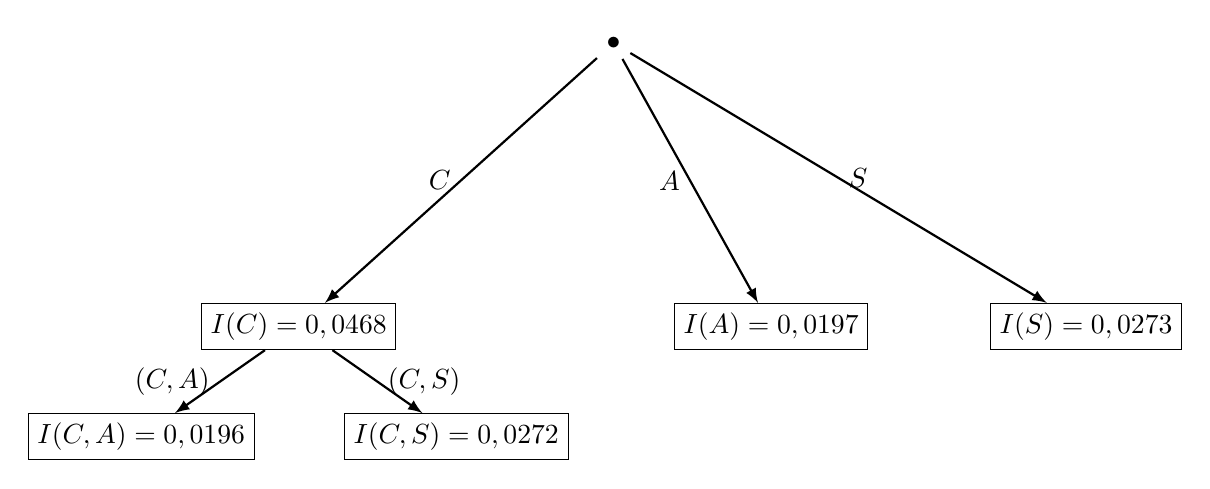
\begin{tikzpicture}[xscale=1,yscale=1]
% Styles (MODIFIABLES)
\tikzstyle{fleche}=[->,>=latex,thick]
\tikzstyle{noeud}=[draw]
\tikzstyle{feuille}=[draw]
\tikzstyle{etiquette}=[midway,fill=white,draw]
% Dimensions (MODIFIABLES)
\def\DistanceInterNiveaux{2}
\def\DistanceInterFeuilles{4}
% Dimensions calculées (NON MODIFIABLES)
\def\NiveauA{(-0)*\DistanceInterNiveaux}
\def\NiveauB{(-1.8)*\DistanceInterNiveaux}
\def\NiveauC{(-2.5)*\DistanceInterNiveaux}
\def\InterFeuilles{(1)*\DistanceInterFeuilles}
% Noeuds (MODIFIABLES : Styles et Coefficients d'InterFeuilles)
\node[] (R) at ({(1.5)*\InterFeuilles},{\NiveauA}) {$\bullet$};
\node[noeud] (Ra) at ({(0.5)*\InterFeuilles},{\NiveauB}) {$I(C)=0,0468$};
\node[feuille] (Raa) at ({(0)*\InterFeuilles},{\NiveauC}) {$I(C,A) = 0,0196$};
\node[feuille] (Rab) at ({(1)*\InterFeuilles},{\NiveauC}) {$I(C,S) = 0,0272$};
\node[feuille] (Rb) at ({(2)*\InterFeuilles},{\NiveauB}) {$I(A) = 0,0197$};
\node[feuille] (Rc) at ({(3)*\InterFeuilles},{\NiveauB}) {$I(S) = 0,0273$};
% Arcs (MODIFIABLES : Styles)
\draw[fleche] (R)--(Ra) node[midway , left] {$C$};
\draw[fleche] (Ra)--(Raa) node[midway , left] {$(C,A)$};
\draw[fleche] (Ra)--(Rab) node[midway , right] {$(C,S)$};
\draw[fleche] (R)--(Rb) node[midway , left] {$A$};
\draw[fleche] (R)--(Rc) node[midway , right] {$S$};
\end{tikzpicture}
\end{center}
	\end{enumerate}

Le choix de la seconde variable de segmentation, n'a pas d'importance, car on commençant par $C$, on a déjà conditionné l'arbre.
\end{enumerate}

\newpage

\textbf{Exercice 3 : Recodage avec nombre de classes fixé :}

Pour effectuer les différents codages, il nous a fallu dans un premier temps diviser par l'effectif total $(72)$ pour déterminer la loi de $(X,Y)$ puis de sommer certaines valeurs du tableau pour obtenir la loi de $Y$.

Le codage ne peut se faire qu'en classes contiguës. On notera dans toute la suite : 
\begin{itemize}
\item[$\bullet$] $\{a\}$ entre $0\%$ ;
\item[$\bullet$] $\{b\}$ entre $0$ et $0,5\%$ ;
\item[$\bullet$] $\{c\}$ entre $0,5$ et $1\%$ ;
\item[$\bullet$] $\{d\}$ entre $1$ et $3\%$ ;
\item[$\bullet$] $\{e\}$ plus de $3\%$.
\end{itemize} 

Les résultats sont arrondis à $10^{-4}$ près.

\begin{enumerate}
\item 
	\begin{enumerate}
	\item \textbf{Codage en deux classes :}
		\begin{itemize}
		\item[$\bullet$] $\{a\};\{b,c,d,e\}$ : $H(X)=-p_a\ln(p_a)-p_{(b,c,d,e)}\ln(p_{(b,c,d,e)}) \approx 0,6741$
		\item[$\bullet$] $\{a,b\};\{c,d,e\}$ : $H(X) \approx 0,6616$
		\item[$\bullet$] $\{a,b,c\};\{d,e\}$ : $H(X) \approx 0,4275$
		\item[$\bullet$] $\{a,b,c,d\};\{e\}$ : $H(X) \approx 0,0732$
		\end{itemize}
Pour le recodage de $X$ en deux classes, on choisira le recodage $\{a\};\{b,c,d,e\}$.
	\item \textbf{Codage en trois classes :}
		\begin{itemize}
		\item[$\bullet$] $\{a\};\{b\};\{c,d,e\}$ : $H(X)=-p_a\ln(p_a)-p_b\ln(p_b)-p_{(c,d,e)}\ln(p_{(c,d,e)}) \approx 1,0683$
		\item[$\bullet$] $\{a,b\};\{c\};\{d,e\} $ : $H(X)\approx 0,9150$
		\item[$\bullet$] $\{a,b,c\};\{d\};\{e\} $ : $H(X)\approx 0,6060$
		\item[$\bullet$] $\{a\};\{b,c\};\{d,e\} $ : $H(X)\approx 0,9412$
		\item[$\bullet$] $\{a\};\{b,c,d\};\{e\} $ : $H(X)\approx 0,8721$
		\item[$\bullet$] $\{a,b\};\{c,d\};\{e\} $ : $H(X)\approx 0,8529$
		\end{itemize}

Pour le recodage de $X$ en trois classes, on choisira le recodage $\{a\};\{b\};\{c,d,e\}$.
	\end{enumerate}

\item \textbf{Recodage en deux classes de $X$ pour la prédiction de $Y$}

A finir, c'est du copier coller en dessous :

%Calculons l'information mutuelle $\displaystyle I(X,Y) = \sum_{x\in X } \sum_{y\in Y} \mathds{P}^{(X,Y)}(x,y) \ln\left(\frac{\mathds{P}^{(X,Y)}(x,y) }{\mathds{P}^{X}(x) \mathds{P}^{Y}(y) }\right)$.

\begin{itemize}
		\item[$\bullet$] $\{a\};\{b,c,d,e\}$ : $I(X,Y)=-p_a\ln(p_a)-p_{(b,c,d,e)}\ln(p_{(b,c,d,e)}) \approx 0,6741$
		\item[$\bullet$] $\{a,b\};\{c,d,e\}$ : $H(X) \approx 0,6616$
		\item[$\bullet$] $\{a,b,c\};\{d,e\}$ : $H(X) \approx 0,4275$
		\item[$\bullet$] $\{a,b,c,d\};\{e\}$ : $H(X) \approx 0,0732$
		\end{itemize}
\end{enumerate}
\end{document}
